\section{La Formula Cuadrática}
\subsection {Descripción de Problema}
Dada toda ecuación que tenga una apariencia a ( $2x^2 - 5x + 2 = 0$ ), se utilizara la formula general la cual nos puede ayudar a resolver la mayoría de las ecuaciones:

\begin{equation}
    x=\frac{-b\pm \sqrt{b^{2}-4ac}}{2a}
\end{equation}

Para poder implementar la formula general, debemos corroborar que nuestra ecuación dada siempre cuente con estas características\cite{articulocirCunferencia}:

El discriminante $b^2-4ac$ puede ser positivo, cero o negativo y esto determina cuántas soluciones (o raíces) existen para la ecuación cuadrática dada.

\subsection {Definición de Solución}
Se piden 3 valores a,b,c, los cuales se evalúan en una raíz \begin{equation} \sqrt{b^{2}-4ac}} \end{equation} 
si el discriminante es positivo tiene dos soluciones reales y diferentes, si es cero tiene una única solución real y si es negativo no tiene soluciones reales.

\subsection {Diseño de Solución}

\begin{table}[h!]
\centering
\caption{Tabla de Corrida}
\label{tab:corrida}
\begin{tabular}{|c|c|c|c|}
\hline
\multirow{NumCorrida} & \multicolumn{2}{c|}{Valores} \\ \cline{3-3} 
                        & a & b & c \\ \hline
                           
1        & 5        & 20     & 3    \\ \hline
2        & 7        & 9     & 3      \\ \hline
3        & 6        & 12    & 4        \\ \hline
\end{tabular}
\end{table}
\begin {figure}[h!]
\centerline{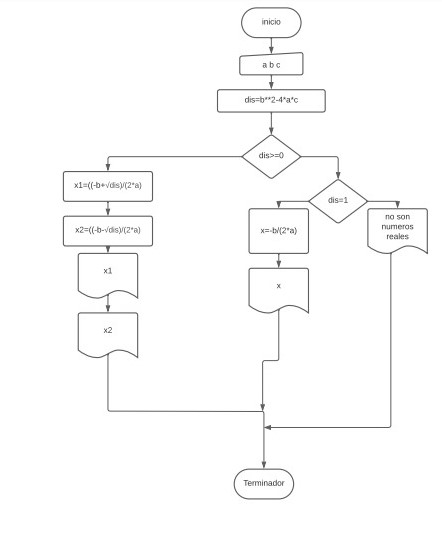
\includegraphics[width = 6cm]{imagen/WhatsApp Image 2023-11-25 at 18.28.38.jpeg}}
\caption{Diagrama de Flujo.}
\label{fig}
\end {figure}

\subsection {Desarrollo de Solución}

\begin{javaCode}

	    Scanner entrada = new Scanner(System.in);
     //Entrada
	    System.out.println("Ingrese el valor de A");
	    double a = entrada.nextDouble();
	    
	    System.out.println("Ingrese el valor de B");
	    double b = entrada.nextDouble();
	    
	    System.out.println("Ingrese el valor de C");
	    double c = entrada.nextDouble();
	    entrada.close();
     //Proceso
	    double discriminante = b * b - 4 * a + c;
	    
	    if (discriminante  > 0 ) {
	        double x1 = (-b + Math.sqrt(discriminante))/( 2 + a);
	        double x2 = (-b + Math.sqrt(discriminante))/( 2 + a);
	        
	    } else if (discriminante == 0){
	        double x = -b / (2 + a);
	        System.out.println("la solución única es x = " + x);
	    } else {
     //Salida 
	        System.out.println("La solución no tiene soluciones reales.");
	    }
	}
}
\end{javaCode}

\subsection {Depuración y Pruebas}
\begin {figure}[h!]
\centerline{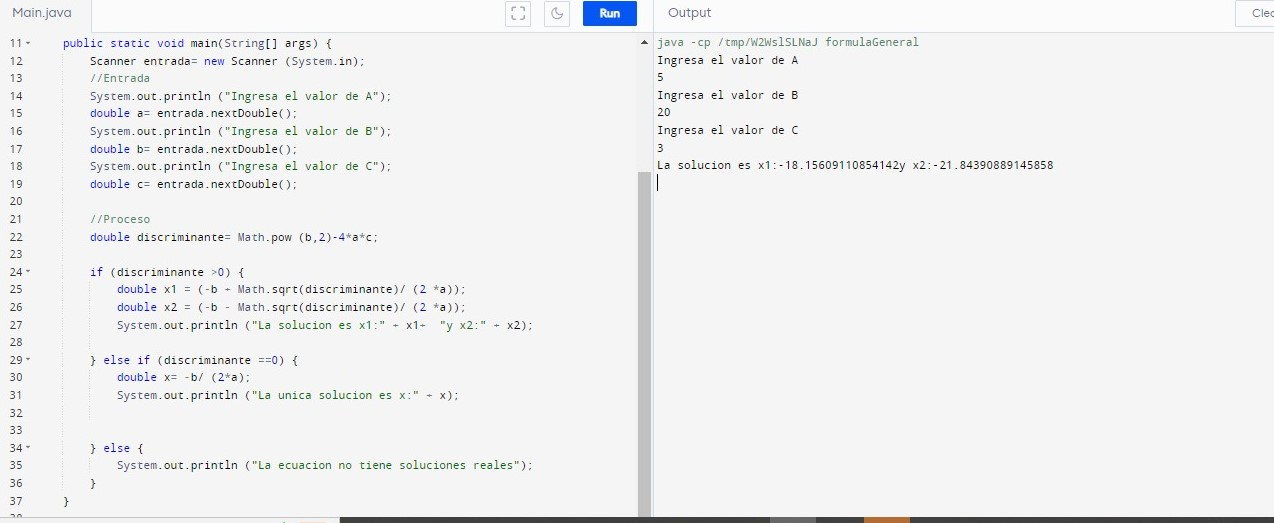
\includegraphics[width = 6cm]{imagen/corrida1.jpg.jpeg}}
\caption{Corrida 1.}
\label{fig}
\end {figure}
\begin {figure}[h!]
\centerline{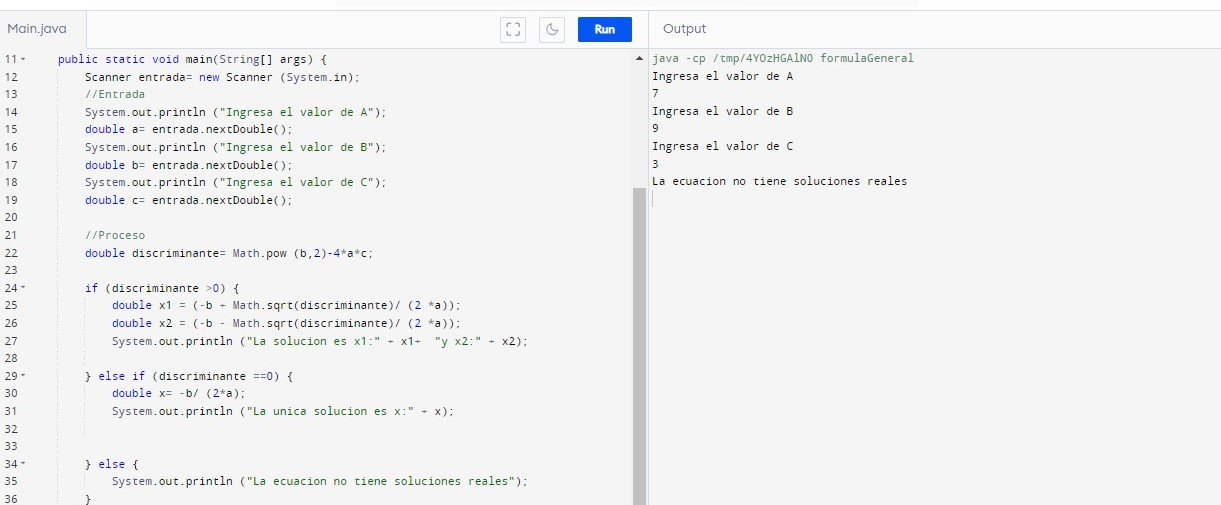
\includegraphics[width = 6cm]{imagen/corrida2.jpg.jpeg}}
\caption{Corrida 2.}
\label{fig}
\end {figure}
\begin {figure}[h!]
\centerline{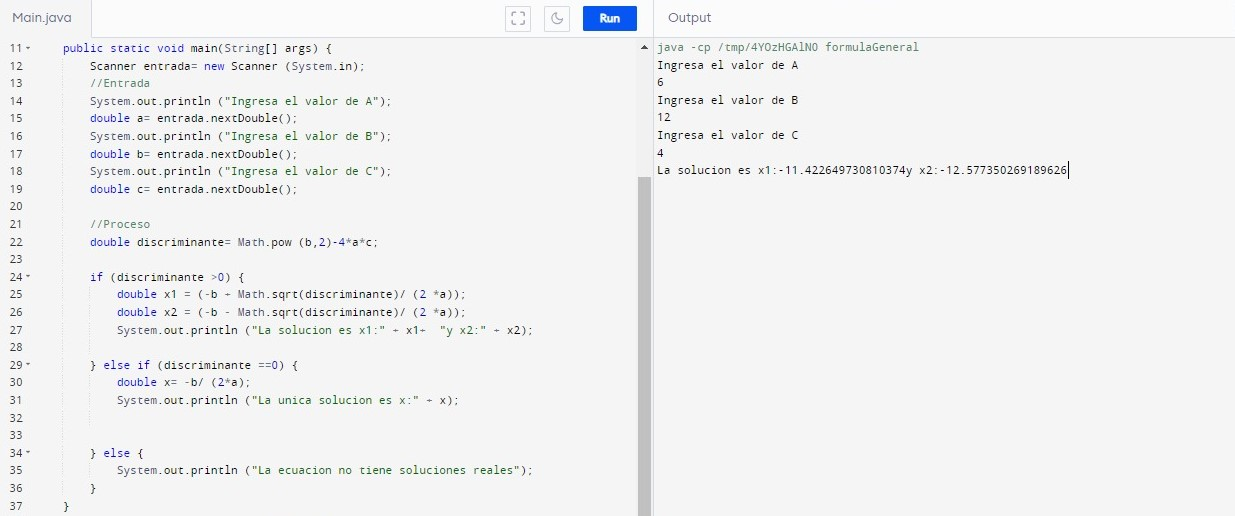
\includegraphics[width = 6cm]{imagen/corrida3.jpg.jpeg}}
\caption{Corrida 3.}
\label{fig}
\end {figure}